\documentclass{article}
\usepackage{graphicx}
\usepackage{indentfirst}
\usepackage{tocloft}
\usepackage{listings}
\usepackage{color}

\definecolor{dkgreen}{rgb}{0,0.6,0}
\definecolor{gray}{rgb}{0.5,0.5,0.5}
\definecolor{mauve}{rgb}{0.58,0,0.82}

\lstset{language=SQL,
  basicstyle={\large\ttfamily},
  belowskip=3mm,
  breakatwhitespace=true,
  breaklines=true,
  classoffset=0,
  columns=flexible,
  commentstyle=\color{dkgreen},
  framexleftmargin=0.25em,
  frameshape={}{yy}{}{}, 
  keywordstyle=\color{blue},
  numbers=none, 
  numberstyle=\tiny\color{gray},
  showstringspaces=false,
  stringstyle=\color{mauve},
  tabsize=3,
  xleftmargin =1em
}

\title{MANAGERIEREA UNUI LANT DE MALL-URI}
\author{Mitu Iustin Aurelian 151}
\date{Septembrie 2023}

\begin{document}
\maketitle
\newpage

\renewcommand{\contentsname}{\centering Cuprins}
\renewcommand{\cftsecleader}{\cftdotfill{\cftdotsep}}
\renewcommand{\cftsecfont}{\bfseries}
\renewcommand{\cftsecpresnum}{\hspace{1em}}
\renewcommand{\cftsecindent}{\cftsecnumwidth}
\renewcommand{\cftsecnumwidth}{2.5em}

\tableofcontents



\addcontentsline{toc}{section}{Exercițiul 1}
\section*{1. Descrierea modelului real, a utilitatii acestuia si a regulilor de functionare.}

\vspace{1cm}

Modelul real va gestiona informatii legate de functionarea unui lant international de mall-uri. Baza de date are scopul de a gestiona informatiile acestor mall-uri . 

Acest lant va cupride mai multe mall-uri din tari diferite. Fiecarui mall i se va tine evidenta asupranumelui si dimensiunii acestuia (in metrii patrati). In interiorul fiecarui mall vor exista mai mute magazine. Magazinele vor emite un profit lunar (calculate in euro) si poate fi contactat prin numarul de telefon asociat. 

Pentru a asigura paza si linistea in interior,
fiecare mall va avea un contrat cu o unica firma de securitate. Firma de securitate va contine angajati responsabili cu paza. Intr-un magazin vor lucre mai multi angajati. Deci, angajatii din aceasta baza de date pot fi doar de 2 tipuri, paznici (din cadrul firmei de securitate) si interni (adica angajatii fiecarui magazin in parte). 

Fiecare magazin va avea mai multe stocuri (in baza mea de date un stoc este vazut mai mult ca o categorie de produse, entitatea produs reprezinta efectiv un singur produs, iar stocul va avea si cantitatea de produse) , care este alcatuit din mai multe produse. Produsul reprezinta bunul material pe care un client il poate procura, sau chiar un serviciu de care clientul poate beneficia. 

Clientii sunt persoane care viziteaza mall-ul pentru a face achizitii.
Acesti client sunt inregistrati in baza de date doar daca fac cel putin o achitie. Totodata, acestia pot efectua mai multe tranzactii in cadrul unui mall, in magazine diferite. Viceversa, un magazine poate vinde produse mai multor client. Orice client are optiunea de a face o reclamatie unui magazin in cazul in care ceva nu pare la locul lui. Pentru a face o relcamatie clientul are nevoie de un motiv (pe care il poate mentiona in reclamatie). 

Detinatorul unui mall se numeste chirias, si acesta poate avea mai multe
magazine inchiriate. El se ocupa cu gestionarea fiecarui magazin pe care il detine, dar si de alte aspecte financiare. 

Un mall poate avea asociata o companie de promovare, dar nu este obligatoriu. Aceasta promovare are o data cand incepe si o data cand se sfarseste. Promovarea are scopul de a face publicitate mall-ului cu telul de a atrage mai multi clienti pentru a genera mai mult profit. 


\addcontentsline{toc}{section}{Exercițiul 2}
\section*{2. Prezentarea constrangerilor (restrictii, reguli) impuse asupra modelului.}
\vspace{1cm}
\begin{itemize}
    \item Nu exista entitatea lant, consideram ca este unul singur, unic.
    \item Exista mai multe mall-uri in acest lant.
    \item Toate mall-urile au cel putin un magazin
    \item O firma de securitate poate semna contractul cu mai multe mall-uri, dar un mall poate avea o singura firma de securitate.
    \item Angajatii din cadrul fiecarui magazin pot fi interni ( tin de magazin in sine) sau de la securitate.
    \item Obligatoriu fiecare magazin detine cel putin un stoc. Fiecare stoc detine produse.
    \item Pot exista mai multi client in cadrul unui magazin, dar fiecare client poate fi clientul mai multor magazine. (Relatie de tip 3)
    \item Clientii nu sunt obligati sa faca tranzactii (sa cumpere produse), si nici sa faca relcamatii.
    \item Fiecare magazin este detinut de un chirias, iar un chirias poate avea mai multe magazine.
    \item Un mall poate avea o campanie de promovare, dar nu e obligatoriu.
    \item Fiecare mall are obligatoriu o firma de securitate afiliata.
\end{itemize}


\addcontentsline{toc}{section}{Exercițiul 3}
\section*{3. Descrierea entitatilor, incluzand precizarea cheii primare.}

\vspace{1cm}

Pentru modelul de date referitor la lantul de mall-uri, structurile MALL, MAGAZIN, FIRMA, PRODUS, CLIENT, ANGAJAT, TRANZACTIE, RECLAMATIE, STOC,
CHIRIAS, PROMOVARE reprezinta entitati.

Toate entitatile sunt independente mai putin entitatea RECLAMATIE (care va
depinde de client si magazinul caruia i s-a atribuit aceasta reclamatie).

\subsection*{\centering ENTITATILE DE BAZA}

Acestea reprezinta substantivele preluate din descrierea bazei de date, entitatile necesare pentru a o prelucra.

\vspace{0.5cm}

\begin{enumerate}
    \item \textbf{MALL}
    - O institutie comerciala ce detine mai multe magazine. Mall-ul are scopul
    de a scoate profit din locurile comerciale inchiriate.

    \begin{itemize}
        \item CHEIE PRIMARA = \textbf{id\_mall}
        \item CHEI STRAINE 
                            \begin{itemize}
                                \item \textbf{id\_firma} care referentiaza tabela FIRMA (id\_firma)
                                \item \textbf{id\_promovare} care referentiaza tabela PROMOVARE (id\_promovare)
                            \end{itemize}
            
    \end{itemize}

    \vspace{0.5cm}
    
    \item \textbf{MAGAZIN}
    - Un spatiu comercial destinat persoanelor publice. In cadrul unui
magazin se realizeaza mai multe tranzactii de catre clienti.

    \begin{itemize}
        \item CHEIE PRIMARA = \textbf{id\_magazin}
        \item CHEI STRAINE 
                            \begin{itemize}
                                \item \textbf{id\_chirias} care referentiaza tabela CHIRIAS (id\_chirias)
                                \item \textbf{id\_mall} care referentiaza tabela MALL (id\_mall)
                            \end{itemize}
            
    \end{itemize}

    \vspace{0.5cm}

    \item \textbf{FIRMA}
    - – Reprezinta firma de securitate. Aceasta are rolul de a mentine linistea
si buna functionare a mall-ului. Acest aspect se realizeaza cu ajutorul angajatilor.

    \begin{itemize}
        \item CHEIE PRIMARA = \textbf{id\_firma}
    \end{itemize}

    \vspace{0.5cm}

    \item \textbf{PRODUS}
    - Un obiect sau serviciu vandut intr-un magazin. Acesta poate fi
achizitionat de un client in urma unei tranzactii.

    \begin{itemize}
        \item CHEIE PRIMARA = \textbf{id\_produs}
        \item CHEI STRAINE 
                            \begin{itemize}
                                \item \textbf{id\_stoc} care referentiaza tabela STOC (id\_stoc)
                                \item \textbf{id\_tranzactie} care referentiaza tabela TRANZACTIE (id\_tranzactie)
                            \end{itemize}
            
    \end{itemize}

        \vspace{0.5cm}

        \item \textbf{CLIENT}
    - Persoana care nu poate fi angajat in acelasi timp. El poate doar sa
viziteze un magazin, nu e obligat sa faca tranzactii.

    \begin{itemize}
        \item CHEIE PRIMARA = \textbf{id\_client}
    \end{itemize}

    \vspace{0.5cm}

    \item \textbf{ANGAJAT}
    - Persoana care poate fi INTERN intr-un magazin , sau PAZNIC de la
firma de securitate. Aceasta este o superentitate.

    \begin{itemize}
        \item CHEIE PRIMARA = \textbf{id\_angajat}    
    \end{itemize}

    \vspace{0.5cm}

    \begin{enumerate}
        \item \textbf{INTERN}
        - Persoana care lucreaza in interiorul unui magazin. Spre exemplu personalul de la casa de marcat sau personalul care se ocupa cu aranjatul hainelor. 

        \begin{itemize}
        \item CHEIE PRIMARA = \textbf{id\_intern}
        \item CHEI STRAINE 
                            \begin{itemize}
                                \item \textbf{id\_angajat} care referentiaza tabela ANGAJAT (id\_angajat)
                                \item \textbf{id\_magazin} care referentiaza tabela MAGAZIN (id\_magazin)
                            \end{itemize}
            
        \end{itemize}

         \vspace{0.5cm}
        
        \item \textbf{PAZNIC}
        - Persoana care lucreaza in interiorul unui mall. Acesta are scopul de a asigura linistea si siguranta clientilor. Acesta este bineinteles in stransa legatura cu firma de securitate la care lucreaza.

        \begin{itemize}
        \item CHEIE PRIMARA = \textbf{id\_paznic}
        \item CHEI STRAINE 
                            \begin{itemize}
                                \item \textbf{id\_angajat} care referentiaza tabela ANGAJAT (id\_angajat)
                                \item \textbf{id\_mall} care referentiaza tabela FIRMA (id\_firma)
                            \end{itemize}
            
        \end{itemize}
    \end{enumerate}

    \vspace{0.5cm}
    
     \item \textbf{TRANZACTIE}
    - Entitate ce contine informatii precum cine a realizat tranzactia,
metoda de plata, ce produse a cumparat, etc.

    \begin{itemize}
        \item CHEIE PRIMARA = \textbf{id\_tranzactie}
            
    \end{itemize}

    \vspace{0.5cm}

    \item \textbf{RECLAMATIE}
    - Entitate ce contine informatii precum cine a realizat reclamatia,
si motivul. Reclamatia poate fi creata doar de un client oricand acesta considera ca are un motiv pentru a face o reclamatie.

    \begin{itemize}
        \item CHEIE PRIMARA (COMPUSA) = \textbf{id\_reclamatie + id\_magazin + id\_client}
        \item CHEI STRAINE 
                            \begin{itemize}
                                \item \textbf{id\_magazin} care referentiaza tabela MAGAZIN (id\_magazin)
                                \item \textbf{id\_client} care referentiaza tabela CLIENT (id\_client)
                            \end{itemize}
            
    \end{itemize}

    \vspace{0.5cm}
    
    \item \textbf{STOC}
    - Entitate ce contine informatii precum cate produse mai sunt valabile,
numarul minim si maxim necesar de produse.

    \begin{itemize}
        \item CHEIE PRIMARA = \textbf{id\_stoc}
        \item CHEIE STRAINA
                            \begin{itemize}
                                \item \textbf{id\_magazin} care referentiaza tabela MAGAZIN (id\_magazin)
                            \end{itemize}
            
    \end{itemize}

    \vspace{0.5cm}

    \item \textbf{CHIRIAS}
    - Persoana care detine cel putin un magazin.
    
    \begin{itemize}
        \item CHEIE PRIMARA = \textbf{id\_chirias}      
    \end{itemize}

    \vspace{0.5cm}

    \item \textbf{PROMOVARE}
    - Reprezinta campania de promovare a unui mall. 

    \begin{itemize}
        \item CHEIE PRIMARA = \textbf{id\_promovare}
    \end{itemize}
    
\end{enumerate}


\subsection*{\centering ENTITATILE ASOCIATIVE}

Acestea reprezinta entitatile create in urma relatiilor de tip 3 sau de tip many-to-many


\begin{enumerate}
    \item \textbf{ACHIZITIE}
    - Aceasta entitate a fost creata in urma relatiei de tip 3 intre entitatile TRANZACTIE, MAGAZIN si CLIENT. Aceasta are scopul de a pastra informatii precum: ce contine produse contine tranzactia, cine a realizat-o si magazinul in care s-a realizat.
    
    \begin{itemize}
        \item CHEIE PRIMARA (COMPUSA) = \textbf{id\_client + id\_magazin + id\_tranzactie}      
    
    \item CHEI STRAINE
                            \begin{itemize}
                                \item \textbf{id\_client} care referentiaza tabela CLIENT (id\_client)
                                \item \textbf{id\_magazin} care referentiaza tabela MAGAZIN (id\_magazin)
                                \item \textbf{id\_tranzactie} care referentiaza tabela TRANZACTIE (id\_tranzactie)
                            \end{itemize}
    \end{itemize}
\end{enumerate}


\addcontentsline{toc}{section}{Exercițiul 4}
\section*{4. Descrierea relatiilor, incluzand precizarea cardinalitatii acestora
}
\vspace{1cm}
\begin{enumerate}
    \item \textbf{MALL} contine \textbf{MAGAZIN}
    \begin{itemize}
        \item Fiecare mall are mai multe magazine afiliate (cel putin 1).
        \item \textbf{1(1):n(1)}
    \end{itemize}
    
    \vspace{0.5cm}

    \item \textbf{MALL} angajeaza \textbf{FIRMA}
    \begin{itemize}
        \item Fiecare mall angajeaza o unica firma de securitate.
        \item Firma de securitate poate lucra la mai multe mall-uri. 
        \item \textbf{1(1):n(1)}
    \end{itemize}

    \vspace{0.5cm}

    \item \textbf{PROMOVARE} promoveaza \textbf{MALL}
    \begin{itemize}
        \item Fiecare mall poate avea o unica campanie de promovare.
        \item Nu e obligatoriu sa aiba una. 
        \item \textbf{1(0):1(1)}
    \end{itemize}

    \vspace{0.5cm}

    \item \textbf{MAGAZIN} detine \textbf{STOC}
    \begin{itemize}
        \item Fiecare magazin are un unic stoc.
        \item \textbf{1(1):1(1)}
    \end{itemize}

    \vspace{0.5cm}

    \item \textbf{MAGAZIN} are \textbf{RECLAMATIE}
    \begin{itemize}
        \item Un magazin poate avea mai multe reclamatii sau deloc.
        \item Nu e obligatoriu sa aiba una. 
        \item \textbf{1(1):1(0)}
    \end{itemize}

    \vspace{0.5cm}

    \item \textbf{CHIRIAS} inchiriaza \textbf{MAGAZIN}
    \begin{itemize}
        \item Un magazin are un unic chirias.
        \item Un chirias poate avea mai multe magazine. 
        \item \textbf{1(1):n(1)}
    \end{itemize}

    \vspace{0.5cm}

    \item \textbf{INTERN} lucreaza \textbf{MAGAZIN}
    \begin{itemize}
        \item Un magazin are mai multi interni.
        \item Un intern poate lucra la un singur magazin. 
        \item \textbf{n(1):1(1)}
    \end{itemize}

    \vspace{0.5cm}

    \item \textbf{TRANZACTIE} exista \textbf{PRODUS}
    \begin{itemize}
        \item Intr-o tranzactie exista unul sau mai multe produse.
        \item \textbf{1(1):n(1)}
    \end{itemize}

    \vspace{0.5cm}

    \item \textbf{STOC} exista \textbf{PRODUS}
    \begin{itemize}
        \item Intr-un stoc exista unul sau mai multe produse.
        \item \textbf{1(1):n(1)}
    \end{itemize}

    \vspace{0.5cm}

    \item \textbf{CLIENT} realizeaza \textbf{RECLAMATIE}
    \begin{itemize}
        \item Un client poate face una sau mai multe reclamatii unui magazin.
        \item \textbf{1(1):n(0)}
    \end{itemize}

    \vspace{0.5cm}

    \item \textbf{PAZNIC} lucreaza \textbf{FIRMA}
    \begin{itemize}
        \item Un paznic lucreaza la o firma de securitate.
        \item Firma detine unul sau mai multi paznici.
        \item \textbf{n(1):1(1)}
    \end{itemize}

    \vspace{0.5cm}

    \item Relatia dintre entitatile \textbf{MAGAZIN}, \textbf{TRANZACTIE}, \textbf{CLIENT} (face)
    \begin{itemize}
        \item Un client poate face mai multe tranzactii din mai multe magazine.
        \item Relatie de tip 3
        \item Relatie ce se realizeaza prin intermediul tabelului asociativ \textbf{ACHIZITIE}
        \item \textbf{n(1):n(1):n(1)}
    \end{itemize}

    \vspace{0.5cm}

    \item \textbf{PAZNIC} este \textbf{ANGAJAT}
    \begin{itemize}
        \item PAZNIC reprezinta subentitatea tabelului ANGAJAT.
        \item \textbf{1(1):1(1)}
    \end{itemize}
    
    \vspace{0.5cm}

    \item \textbf{INTERN} este \textbf{ANGAJAT}
    \begin{itemize}
        \item INTERN reprezinta subentitatea tabelului ANGAJAT.
        \item \textbf{1(1):1(1)}
    \end{itemize}
    
\end{enumerate}


\addcontentsline{toc}{section}{Exercițiul 5}
\section*{5. Descrierea atributelor, incluzand tipul de date si eventualele constrangeri, valori implicite, valori posibile ale atributelor.}
\vspace{1cm}
\begin{enumerate}

    \item \textbf{MALL}
    \begin{itemize}
    
        \item \textbf{id\_mall }
                \begin{itemize}
                    \item Descriere: Reprezinta identificatorul unic al mall-ului.
                    \item Tip de date: NUMBER(4)
                    \item Constrangeri: CHEIE PRIMARA, NOT NULL
                \end{itemize}
                
        \item \textbf{tara}
                \begin{itemize}
                    \item Descriere: Reprezinta tara in care este situat mall-ul.
                    \item Tip de date: VARCHAR2(50)
                    \item Constrangeri: -
                \end{itemize}

        \item \textbf{nume\_mall}
                \begin{itemize}
                    \item Descriere: Reprezinta numele mall-ul.
                    \item Tip de date: VARCHAR2(50)
                    \item Constrangeri: -
                \end{itemize}
                
        \item \textbf{dimensiune}
                \begin{itemize}
                    \item Descriere: Reprezinta dimensiunea mall-ul in $m^{2}$.
                    \item Tip de date: NUMBER(4)
                    \item Constrangeri: -
                \end{itemize}

        \item \textbf{id\_firma}
                \begin{itemize}
                    \item Descriere: Reprezinta cheie ce referentiaza tabelul FIRMA (id\_firma) .
                    \item Tip de date: NUMBER(4)
                    \item Constrangeri: CHEIE STRAINA 
                \end{itemize}

        \item \textbf{id\_promovare}
                \begin{itemize}
                    \item Descriere: Reprezinta cheie ce referentiaza tabelul PROMOVARE (id\_promovare) .
                    \item Tip de date: NUMBER(4)
                    \item Constrangeri: CHEIE STRAINA 
                \end{itemize}
                
    \end{itemize}

    \vspace{0.5cm}

    \item \textbf{FIRMA}
    \begin{itemize}
    
        \item \textbf{id\_firma }
                \begin{itemize}
                    \item Descriere: Reprezinta identificatorul unic al firmei.
                    \item Tip de date: NUMBER(4)
                    \item Constrangeri: CHEIE PRIMARA, NOT NULL
                \end{itemize}
                
        \item \textbf{nume\_firma}
                \begin{itemize}
                    \item Descriere: Reprezinta numele firmei.
                    \item Tip de date: VARCHAR2(50)
                    \item Constrangeri: -
                \end{itemize}
                
    \end{itemize}

    \vspace{0.5cm}


    \item \textbf{PROMOVARE}
    \begin{itemize}
    
        \item \textbf{id\_promovare }
                \begin{itemize}
                    \item Descriere: Reprezinta identificatorul unic al campaniei de promovare.
                    \item Tip de date: NUMBER(4)
                    \item Constrangeri: CHEIE PRIMARA, NOT NULL
                \end{itemize}
                
        \item \textbf{nume\_campanie}
                \begin{itemize}
                    \item Descriere: Reprezinta numele campaniei.
                    \item Tip de date: VARCHAR2(50)
                    \item Constrangeri: -
                \end{itemize}

        \item \textbf{data\_inceput}
                \begin{itemize}
                    \item Descriere: Reprezinta data la care incepe campania de promovare (zi, luna, an).
                    \item Tip de date: DATE
                    \item Constrangeri: -
                \end{itemize}

        \item \textbf{data\_sfarsit}
                \begin{itemize}
                    \item Descriere: Reprezinta data la care se termina campania de promovare (zi, luna, an).
                    \item Tip de date: DATE
                    \item Constrangeri: -
                \end{itemize}
    \end{itemize}

    \vspace{0.5cm}

    \item \textbf{CHIRIAS}
    \begin{itemize}
    
        \item \textbf{id\_chirias}
                \begin{itemize}
                    \item Descriere: Reprezinta identificatorul unic al chiriasului.
                    \item Tip de date: NUMBER(4)
                    \item Constrangeri: CHEIE PRIMARA, NOT NULL
                \end{itemize}
                
        \item \textbf{nume\_chirias}
                \begin{itemize}
                    \item Descriere: Reprezinta numele chiriasului.
                    \item Tip de date: VARCHAR2(50)
                    \item Constrangeri: -
                \end{itemize}

        \item \textbf{email}
                \begin{itemize}
                    \item Descriere: Reprezinta email-ul chiriasului.
                    \item Tip de date: VARCHAR2(30)
                    \item Constrangeri: NOT NULL
                \end{itemize}

    \end{itemize}

    \vspace{0.5cm}

    \item \textbf{MAGAZIN}
    \begin{itemize}
    
        \item \textbf{id\_magazin}
                \begin{itemize}
                    \item Descriere: Reprezinta identificatorul unic al magazinului.
                    \item Tip de date: NUMBER(4)
                    \item Constrangeri: CHEIE PRIMARA, NOT NULL
                \end{itemize}
                
        \item \textbf{nume\_magazin}
                \begin{itemize}
                    \item Descriere: Reprezinta numele magazinului.
                    \item Tip de date: VARCHAR2(50)
                    \item Constrangeri: -
                \end{itemize}

        \item \textbf{telefon}
                \begin{itemize}
                    \item Descriere: Reprezinta numarul de telefon al chiriasului.
                    \item Tip de date: VARCHAR2(30)
                    \item Constrangeri: NOT NULL
                \end{itemize}

        \item \textbf{profit\_lunar}
                \begin{itemize}
                    \item Descriere: Reprezinta profitul lunar facut de magazin.
                    \item Tip de date: NUMBER(7)
                    \item Constrangeri: -
                \end{itemize}


        \item \textbf{id\_chirias}
                \begin{itemize}
                    \item Descriere: Reprezinta cheie ce referentiaza tabelul CHIRIAS (id\_chirias).
                    \item Tip de date: NUMBER(4)
                    \item Constrangeri: CHEIE STRAINA, NOT NULL
                \end{itemize}

        \item \textbf{id\_mall}
                \begin{itemize}
                    \item Descriere: Reprezinta cheie ce referentiaza tabelul MALL (id\_mall).
                    \item Tip de date: NUMBER(4)
                    \item Constrangeri: CHEIE STRAINA, NOT NULL
                \end{itemize}
    \end{itemize}

    \vspace{0.5cm}

    \item \textbf{STOC}
    \begin{itemize}
    
        \item \textbf{id\_stoc}
                \begin{itemize}
                    \item Descriere: Reprezinta identificatorul unic al stocului.
                    \item Tip de date: NUMBER(4)
                    \item Constrangeri: CHEIE PRIMARA, NOT NULL
                \end{itemize}
                
       \item \textbf{id\_magazin}
                \begin{itemize}
                    \item Descriere: Reprezinta cheie ce referentiaza tabelul MAGAZIN (id\_magazin).
                    \item Tip de date: NUMBER(4)
                    \item Constrangeri: CHEIE STRAINA, NOT NULL
                \end{itemize}

    \end{itemize}

    \vspace{0.5cm}

    \item \textbf{TRANZACTIE}
    \begin{itemize}
    
        \item \textbf{id\_tranzactie}
                \begin{itemize}
                    \item Descriere: Reprezinta identificatorul unic al tranzactiei.
                    \item Tip de date: NUMBER(4)
                    \item Constrangeri: CHEIE PRIMARA, NOT NULL
                \end{itemize}
                
       \item \textbf{data\_ora}
                \begin{itemize}
                    \item Descriere: Reprezinta data si ora la care a fost facuta tranzactia.
                    \item Tip de date: TIMPESTAMP
                    \item Constrangeri: -
                \end{itemize}

    \end{itemize}

    \vspace{0.5cm}

    \item \textbf{PRODUS}
    \begin{itemize}
    
        \item \textbf{id\_produs}
                \begin{itemize}
                    \item Descriere: Reprezinta identificatorul unic al produsului.
                    \item Tip de date: NUMBER(4)
                    \item Constrangeri: CHEIE PRIMARA, NOT NULL
                \end{itemize}

        \item \textbf{nume\_produs}
                \begin{itemize}
                    \item Descriere: Reprezinta numele produsului.
                    \item Tip de date: VARCHAR2(50)
                    \item Constrangeri: -
                \end{itemize}

        \item \textbf{pret}
                \begin{itemize}
                    \item Descriere: Reprezinta pretul produsului.
                    \item Tip de date: NUMBER(4)
                    \item Constrangeri: -
                \end{itemize}
                
       \item \textbf{id\_stoc}
                \begin{itemize}
                    \item Descriere: Reprezinta cheie ce referentiaza tabelul STOC (id\_stoc).
                    \item Tip de date: NUMBER(4)
                    \item Constrangeri: CHEIE STRAINA
                \end{itemize}

        \item \textbf{id\_tranzactie}
                \begin{itemize}
                    \item Descriere: Reprezinta cheie ce referentiaza tabelul TRANZACTIE (id\_tranzactie).
                    \item Tip de date: NUMBER(4)
                    \item Constrangeri: CHEIE STRAINA
                \end{itemize}
                
    \end{itemize}

    \vspace{0.5cm}

    \item \textbf{CLIENT}
    \begin{itemize}
    
        \item \textbf{id\_client}
                \begin{itemize}
                    \item Descriere: Reprezinta identificatorul unic al clientului.
                    \item Tip de date: NUMBER(4)
                    \item Constrangeri: CHEIE PRIMARA, NOT NULL
                \end{itemize}

        \item \textbf{nume\_client}
                \begin{itemize}
                    \item Descriere: Reprezinta numele clientului.
                    \item Tip de date: VARCHAR2(40)
                    \item Constrangeri: -
                \end{itemize}
        \item \textbf{email}
                \begin{itemize}
                    \item Descriere: Reprezinta email-ul clientului.
                    \item Tip de date: VARCHAR2(30)
                    \item Constrangeri: NOT NULL
                \end{itemize}

        \item \textbf{telefon}
                \begin{itemize}
                    \item Descriere: Reprezinta numarul de telefon al clientului.
                    \item Tip de date: VARCHAR2(14)
                    \item Constrangeri: -
                \end{itemize}

    \end{itemize}

    \vspace{0.5cm}

    \item \textbf{RECLAMATIE}
    \begin{itemize}
    
        \item \textbf{id\_reclamatie}
                \begin{itemize}
                    \item Descriere: Reprezinta identificatorul unic al reclamatiei.
                    \item Tip de date: NUMBER(4)
                    \item Constrangeri: CHEIE PRIMARA, NOT NULL
                \end{itemize}

        \item \textbf{data\_ora}
                \begin{itemize}
                    \item Descriere: Reprezinta data si ora la care a fost facuta reclamatia.
                    \item Tip de date: TIMESTAMP
                    \item Constrangeri: -
                \end{itemize}

        \item \textbf{motiv}
                \begin{itemize}
                    \item Descriere: Reprezinta motivul pentru care a fost facuta reclamatia.
                    \item Tip de date: VARCHAR2(1000)
                    \item Constrangeri: -
                \end{itemize}
                
       \item \textbf{id\_magazin}
                \begin{itemize}
                    \item Descriere: Reprezinta cheie ce referentiaza tabelul MAGAZIN (id\_magazin).
                    \item Tip de date: NUMBER(4)
                    \item Constrangeri: CHEIE STRAINA, NOT NULL
                \end{itemize}

        \item \textbf{id\_client}
                \begin{itemize}
                    \item Descriere: Reprezinta cheie ce referentiaza tabelul CLIENT (id\_client).
                    \item Tip de date: NUMBER(4)
                    \item Constrangeri: CHEIE STRAINA, NOT NULL
                \end{itemize}

    \end{itemize}

    \vspace{0.5cm}

    \item \textbf{ACHIZITIE}
    \begin{itemize}
    
       \item \textbf{id\_magazin}
                \begin{itemize}
                    \item Descriere: Reprezinta cheie ce referentiaza tabelul MAGAZIN (id\_magazin).
                    \item Tip de date: NUMBER(4)
                    \item Constrangeri: CHEIE STRAINA, NOT NULL
                \end{itemize}

        \item \textbf{id\_client}
                \begin{itemize}
                    \item Descriere: Reprezinta cheie ce referentiaza tabelul CLIENT (id\_client).
                    \item Tip de date: NUMBER(4)
                    \item Constrangeri: CHEIE STRAINA, NOT NULL
                \end{itemize}

        \item \textbf{id\_tranzactie}
                \begin{itemize}
                    \item Descriere: Reprezinta cheie ce referentiaza tabelul TRANZACTIE (id\_tranzactie).
                    \item Tip de date: NUMBER(4)
                    \item Constrangeri: CHEIE STRAINA, NOT NULL
                \end{itemize}

    \end{itemize}

    \vspace{0.5cm}

    \item \textbf{ANGAJAT}
    \begin{itemize}
    
        \item \textbf{id\_angajat}
                \begin{itemize}
                    \item Descriere: Reprezinta identificatorul unic al angajatului.
                    \item Tip de date: NUMBER(4)
                    \item Constrangeri: CHEIE PRIMARA, NOT NULL
                \end{itemize}

        \item \textbf{nume\_angajat}
                \begin{itemize}
                    \item Descriere: Reprezinta numele angajatului.
                    \item Tip de date: VARCHAR2(30)
                    \item Constrangeri: -
                \end{itemize}

        \item \textbf{salariu}
                \begin{itemize}
                    \item Descriere: Reprezinta salariulin lei al angajatului.
                    \item Tip de date: NUMBER(4)
                    \item Constrangeri: -
                \end{itemize}
                
       \item \textbf{data\_angajarii}
                \begin{itemize}
                    \item Descriere: Reprezinta data la care a fost angajat salariatul.
                    \item Tip de date: DATE
                    \item Constrangeri: -
                \end{itemize}

    \end{itemize}

    \vspace{0.5cm}

    \item \textbf{PAZNIC}
    \begin{itemize}
    
        \item \textbf{id\_paznic}
                \begin{itemize}
                    \item Descriere: Reprezinta identificatorul unic al paznicului.
                    \item Tip de date: NUMBER(4)
                    \item Constrangeri: CHEIE PRIMARA, NOT NULL
                \end{itemize}

        \item \textbf{norma}
                \begin{itemize}
                    \item Descriere: Reprezinta programul paznicului, care poate fi part-time sau full-time (adica norma intreaga).
                    \item Tip de date: VARCHAR2(20);
                    \item Constrangeri: -
                \end{itemize}
                
       \item \textbf{id\_angajat}
                \begin{itemize}
                    \item Descriere: Reprezinta cheie ce referentiaza tabelul ANGAJAT (id\_angajat).
                    \item Tip de date: NUMBER(4)
                    \item Constrangeri: CHEIE STRAINA, UNIQUE
                \end{itemize}

        \item \textbf{id\_firma}
                \begin{itemize}
                    \item Descriere: Reprezinta cheie ce referentiaza tabelul FIRMA (id\_firma).
                    \item Tip de date: NUMBER(4)
                    \item Constrangeri: CHEIE STRAINA
                \end{itemize}

    \end{itemize}

    \vspace{0.5cm}

    \item \textbf{INTERN}
    \begin{itemize}
    
        \item \textbf{id\_intern}
                \begin{itemize}
                    \item Descriere: Reprezinta identificatorul unic al intern-ului.
                    \item Tip de date: NUMBER(4)
                    \item Constrangeri: CHEIE PRIMARA, NOT NULL
                \end{itemize}

        \item \textbf{tura}
                \begin{itemize}
                    \item Descriere: Reprezinta programul intern-ului, care poate fi de zi sau sau de noapte.
                    \item Tip de date: VARCHAR2(20);
                    \item Constrangeri: -
                \end{itemize}
                
       \item \textbf{id\_angajat}
                \begin{itemize}
                    \item Descriere: Reprezinta cheie ce referentiaza tabelul ANGAJAT (id\_angajat).
                    \item Tip de date: NUMBER(4)
                    \item Constrangeri: CHEIE STRAINA, UNIQUE
                \end{itemize}

        \item \textbf{id\_magazin}
                \begin{itemize}
                    \item Descriere: Reprezinta cheie ce referentiaza tabelul MAGAZIN (id\_magazin).
                    \item Tip de date: NUMBER(4)
                    \item Constrangeri: CHEIE STRAINA
                \end{itemize}

    \end{itemize}
    
\end{enumerate}


\addcontentsline{toc}{section}{Exercițiul 6}
\section*{6. Realizarea diagramei entitate-relatie corespunzatoare descrierii de la punctele 3-5}
\vspace{1cm}
\begin{figure}[h]
  \centerline{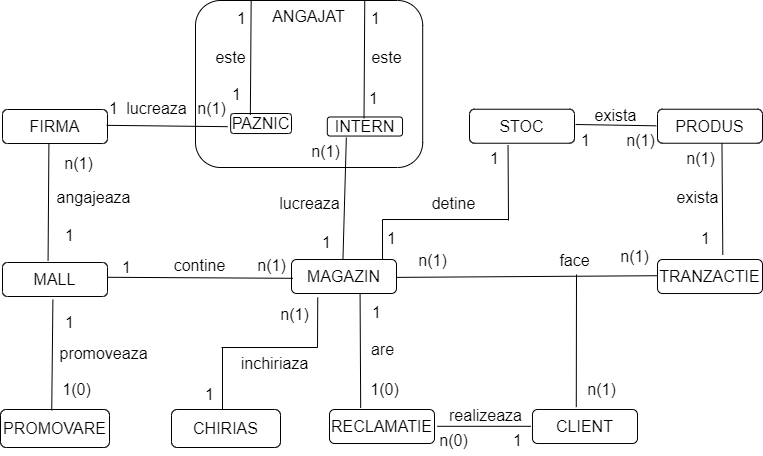
\includegraphics[scale=0.75]{images/ERDSCHEMA.png}}
  \caption{ Diagrama entitate - relatie.}
\end{figure}


\addcontentsline{toc}{section}{Exercițiul 7}
\section*{7. Realizarea diagramei conceptuale corespunzatoare diagramei entitate-relatie proiectata la punctul 6}
\vspace{1cm}
\begin{figure}[h]
  \centerline{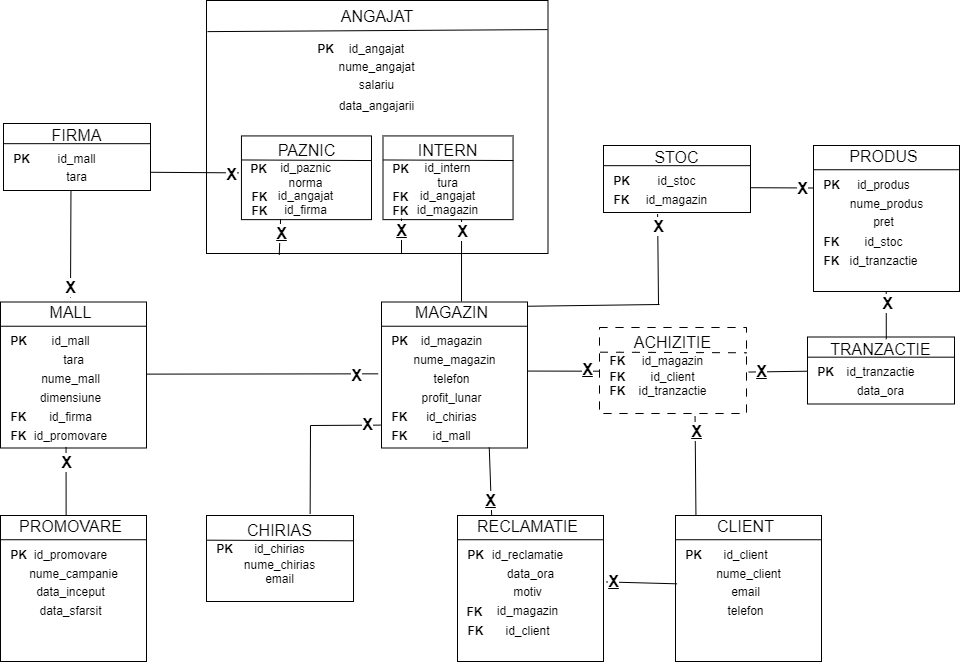
\includegraphics[scale=0.6]{images/CONCEPTUALA.png}}
  \caption{ Diagrama conceptuala.}
\end{figure}


\addcontentsline{toc}{section}{Exercițiul 8}
\section*{8. Enumerarea schemelor relationale corespunzatoare diagramei conceptuale.}

\vspace{1cm}

\begin{itemize}
    \item \textbf{FIRMA} (id\_firma, nume\_firma)
    \item \textbf{MALL} (id\_mall, tara, nume\_mall, dimensiune, id\_firma, id\_promovare)
    \item \textbf{PROMOVARE} (id\_promovare, nume\_campanie, data\_inceput, data\_sfarsit)
    \item \textbf{MAGAZIN} (id\_magazin, nume\_magazin, telefon, profit\_lunar, id\_chirias, id\_mall)
    \item \textbf{ANGAJAT} (id\_angajat, nume\_angajat, salariu, data\_angajarii)
    \item \textbf{PAZNIC} (id\_paznic, norma, id\_angajat, id\_firma)
    \item \textbf{INTERN} (id\_intern, tura, id\_angajat, id\_magazin)
    \item \textbf{CHIRIAS} (id\_chirias, nume\_chirias, email)
    \item \textbf{RECLAMATIE} (id\_reclamatie, data\_ora, motiv, id\_magazin, id\_client)
    \item \textbf{CLIENT} (id\_client, nume\_client, email, telefon)
    \item \textbf{TRANZACTIE} (id\_tranzactie, data\_ora)
    \item \textbf{ACHIZITIE} (id\_client, id\_magazin, id\_tranzactie)
    \item \textbf{PRODUS} (id\_produs, nume\_produs, pret, id\_stoc, id\_tranzactie)
    \item \textbf{STOC} (id\_stoc, id\_magazin)
\end{itemize}


\addcontentsline{toc}{section}{Exercițiul 9}
\section*{9. Realizarea normalizarii pana la forma normala (FN1-FN3).}

\vspace{1cm}

\centering \textbf{FN1}

\vspace{0.2cm}

Avand in vedere faptul ca in baza de date proiectata o firma poate lucra la mai multe mall-uri se putea ca tabelul FIRMA, pe langa atributele id\_firma, nume\_firma, mai putea avea o lista care reprezenta mall-urile la care lucreaza. Acesta situatie incalca Forma Normala 1 deoarece unui atribut ii corespundeau mai multe valori. Astfel, solutia a fost sa creez o cheie straina in tabelul MALL. Aceasta cheie straina este cheia primara din tabelul FIRMA, si astfel fiecarui atribut ii corespunde o valoare indivizibila. 

\vspace{0.5cm}

\textbf{FN2}

\vspace{0.2cm}

In baza de date se poate observa entitatea ANGAJAT. Un caz ipotetic de proiectare, ar fi fost sa construiesc o singura entitate numita ANGAJAT care sa contina toate atributele (si cele de la INTERN si cele de la PAZNIC). In cazul in care angajatul in sine era un paznic spre exemplu, la altributele referitoare la “intern” aveam doar null, si vice-versa. Aceasta proiectare nu respecta Forma Normala 2 deoarece aduce redundanta, si un atribut ar depinde partial de cheia primara( alcatuita atunci din id\_angajat, id\_intern si id\_paznic) . Solutia a fost sa creez superentitatea ANGAJAT unde sa pastrez cateva atribute comune, si
subentitatile INTERN si PAZNIC. Totodata, aceaste relatii dintre PAZNIC/INTERN si
ANGAJAT sunt in FN1 deoarece fiecarui atribut ii corespunde o valoare indivizibila. Astfel, baza de date proiectata se afla in FN2 deoarece fiecare atribut (care nu participa la cheia primara) este dependent de intreaga cheie primara (si atributele din PAZNIC, dar si cele din INTERN).

\vspace{0.5cm}

\textbf{FN3}

\vspace{0.2cm}

In exemplul meu, in entitatea MAGAZIN, pe langa atributele magazinului deja
existente (id\_magazin, nume\_magazin, telefon, profit\_lunar, id\_chirias, id\_mall) as mai fi putut adauga si atributele id\_chirias, nume\_chirias, email\_chirias, etc. Problema ar fi fost ca unele atribute (care nu erau chei) depindeau partial de cheia primara , si nu depindeau in intregime de cheia primara SI DOAR de aceasta. Astfel, aceasta entitate respecta FN1 (deoarece fiecarui atribut ii corespunde o valoare indivizibila, si nu respecta
nici FN2 (deoarece atributele depindeau partial) si nici FN3. Solutia pentru a aduce aceasta entitate in FN3 a fost sa creez entitatea CHIRIAS si sa mut atributele dependente de id\_chirias (adica atributele nume\_chirias si email\_chirias) in noua entitate creata. Acum se respecta FN3 deoarece toate atrbutele depind integral de cheia primara si DOAR de aceasta. 



\addcontentsline{toc}{section}{Exercițiul 10}
\section*{10. Crearea unei secvente ce va fi utilizata in inserarea inregistrarilor in tabele.}


\vspace{1cm}

\begin{lstlisting}
CREATE SEQUENCE SEQ
    INCREMENT BY 1
    START WITH 1
    MAXVALUE 9999
    NOCYCLE;
    
\end{lstlisting}


\addcontentsline{toc}{section}{Exercițiul 11}
\section*{11. Crearea tabelelor in SQL si inserarea de date coerente in fiecare dintre acestea.}

\vspace{1cm}

\begin{itemize}

    \item \textbf{FIRMA}
    \vspace{0.2cm}
    \begin{lstlisting}
CREATE TABLE FIRMA (
 id_firma NUMBER(4) PRIMARY KEY,
 nume_firma VARCHAR2(50)
 );
INSERT INTO FIRMA VALUES (1, 'BGS');
INSERT INTO FIRMA VALUES (2, 'Carpat Guard');
INSERT INTO FIRMA VALUES (3, 'SSG Security');
INSERT INTO FIRMA VALUES (4, 'Tiger Security');
INSERT INTO FIRMA VALUES (5, 'Romanian Security');
    \end{lstlisting}
    \vspace{0.2cm}
    \begin{figure}[h]
      \centerline{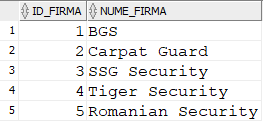
\includegraphics{images/inserare1.png}}
      \caption{ Inserare 1.}
    \end{figure}
    \vspace{0.5cm}
    
    \item \textbf{PROMOVARE}
    \vspace{0.2cm}
    \begin{lstlisting}
CREATE TABLE PROMOVARE (
 id_promovare NUMBER(4) PRIMARY KEY,
 nume_campanie VARCHAR2(50) ,
 data_inceput DATE ,
 data_sfarsit DATE);

INSERT INTO PROMOVARE (id_promovare, nume_campanie, data_inceput, data_sfarsit)
VALUES (1, 'Campania de primavara', TO_DATE('2023-03-15', 'YYYY-MM-DD'), TO_DATE('2023-04-
30', 'YYYY-MM-DD'));
INSERT INTO PROMOVARE (id_promovare, nume_campanie, data_inceput, data_sfarsit)
VALUES (2, 'Campania de reduceri', TO_DATE('2023-09-01', 'YYYY-MM-DD'), TO_DATE('2023-09-15',
'YYYY-MM-DD'));
INSERT INTO PROMOVARE (id_promovare, nume_campanie, data_inceput, data_sfarsit)
VALUES (3, 'Campania de Craciun', TO_DATE('2023-12-10', 'YYYY-MM-DD'), TO_DATE('2023-12-25',
'YYYY-MM-DD'));
INSERT INTO PROMOVARE (id_promovare, nume_campanie, data_inceput, data_sfarsit)
VALUES (4, 'Campania de Paste', TO_DATE('2023-03-01', 'YYYY-MM-DD'), TO_DATE('2023-08-31',
'YYYY-MM-DD'));
INSERT INTO PROMOVARE (id_promovare, nume_campanie, data_inceput, data_sfarsit)
VALUES (5, 'Campania de toamna', TO_DATE('2023-09-15', 'YYYY-MM-DD'), TO_DATE('2023-10-31',
'YYYY-MM-DD'));
    \end{lstlisting} 
    \vspace{0.2cm}
    \begin{figure}[h]
      \centerline{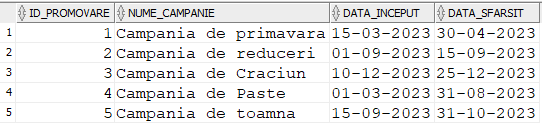
\includegraphics{images/inserare2.png}}
      \caption{ Inserare 2.}
    \end{figure}
    \vspace{0.5cm}

    \item \textbf{MALL}
    \vspace{0.2cm}
    \begin{lstlisting}
CREATE TABLE MALL (
 id_mall NUMBER(4) PRIMARY KEY,
 tara VARCHAR2(50),
 nume_mall VARCHAR2(50),
 dimensiune NUMBER(7),
 id_firma NUMBER(4) NOT NULL,
 id_promovare NUMBER(4),
 FOREIGN KEY (id_firma) REFERENCES FIRMA (id_firma),
 FOREIGN KEY (id_promovare) REFERENCES PROMOVARE (id_promovare)
);
INSERT INTO MALL VALUES (1, 'Romania', 'MegaMall', 10000, 3, 2);
INSERT INTO MALL VALUES (2, 'Spania', 'Plaza Central', 8000, 1, 4);
INSERT INTO MALL VALUES (3, 'Germania', 'City Mall', 12000, 2, 1);
INSERT INTO MALL VALUES (4, 'Franta', 'Le Grand Centre', 15000, 5, 3);
INSERT INTO MALL VALUES (5, 'Italia', 'Fashion Mall', 9000, 4, 5);
INSERT INTO MALL VALUES(6,'Romania','Braila Mall',500,1,null);
    \end{lstlisting}
    \vspace{0.2cm}
    \begin{figure}[h]
      \centerline{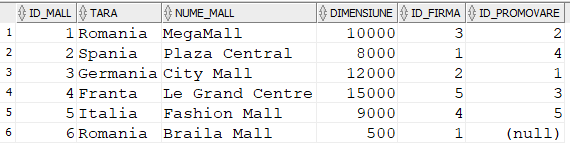
\includegraphics{images/inserare3.png}}
      \caption{ Inserare 3.}
    \end{figure}
    \vspace{0.5cm}

    \item \textbf{CHIRIAS}
    \vspace{0.2cm}
    \begin{lstlisting}
CREATE TABLE CHIRIAS (
 id_chirias NUMBER(4) PRIMARY KEY,
 nume_chirias VARCHAR2(30) ,
 email VARCHAR2(30) NOT NULL
);
INSERT INTO CHIRIAS VALUES (1, 'John Doe', 'john.doe@example.com');
INSERT INTO CHIRIAS VALUES (2, 'Jane Smith', 'jane.smith@example.com');
INSERT INTO CHIRIAS VALUES (3, 'Alex Johnson', 'alex.johnson@example.com');
INSERT INTO CHIRIAS VALUES (4, 'Emily Davis', 'emily.davis@example.com');
INSERT INTO CHIRIAS VALUES (5, 'Michael Brown', 'michael.brown@example.com');
    \end{lstlisting}
    \vspace{0.2cm}
    \begin{figure}[h]
      \centerline{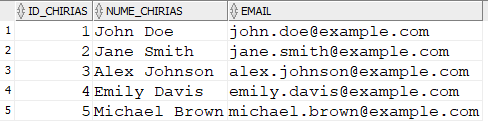
\includegraphics{images/inserare4.png}}
      \caption{ Inserare 4.}
    \end{figure}
    \vspace{0.5cm}

    \item \textbf{MAGAZIN}
    \vspace{0.2cm}
    \begin{lstlisting}
CREATE TABLE MAGAZIN(
 id_magazin NUMBER(4) PRIMARY KEY,
 nume_magazin VARCHAR2(30) ,
 telefon VARCHAR2(30) NOT NULL,
 profit_lunar NUMBER(7),
 id_chirias NUMBER(4) NOT NULL,
 id_mall NUMBER(4) NOT NULL,
 FOREIGN KEY (id_chirias) REFERENCES CHIRIAS (id_chirias),
 FOREIGN KEY (id_mall) REFERENCES MALL (id_mall)
);
INSERT INTO MAGAZIN VALUES (1, 'Carrefour', '123456789', 5000, 1, 1);
INSERT INTO MAGAZIN VALUES (2, 'H and M', '987654321', 7000, 2, 1);
INSERT INTO MAGAZIN VALUES (3, 'New Yorker', '111222333', 6000, 3, 2);
INSERT INTO MAGAZIN VALUES (4, 'Zara', '444555666', 4000, 4, 2);
INSERT INTO MAGAZIN VALUES (5, 'Pull and Bear', '777888999', 8000, 5, 3);
    \end{lstlisting}
    \vspace{0.2cm}
    \begin{figure}[h]
      \centerline{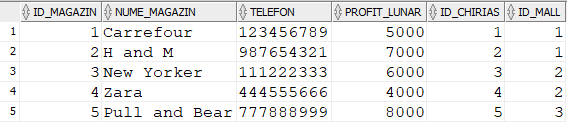
\includegraphics{images/inserare5.png}}
      \caption{ Inserare 5.}
    \end{figure}
    \vspace{0.5cm}

    \item \textbf{STOC}
    \vspace{0.2cm}
    \begin{lstlisting}
CREATE TABLE STOC (
 id_stoc NUMBER(4) PRIMARY KEY,
 id_magazin NUMBER(4),
 FOREIGN KEY (id_magazin) REFERENCES MAGAZIN(id_magazin)
 );

INSERT INTO STOC VALUES (1, 5);
INSERT INTO STOC VALUES (2, 2);
INSERT INTO STOC VALUES (3, 3);
INSERT INTO STOC VALUES (4, 4);
INSERT INTO STOC VALUES (5, 1);
    \end{lstlisting}
    \vspace{4cm}
    \begin{figure}[h]
      \centerline{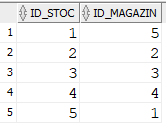
\includegraphics{images/inserare6.png}}
      \caption{ Inserare 6.}
    \end{figure}
    \vspace{0.5cm}

    \item \textbf{TRANZACTIE}
    \vspace{0.2cm}
    \begin{lstlisting}
CREATE TABLE TRANZACTIE(
 id_tranzactie NUMBER(4) PRIMARY KEY,
 data_ora TIMESTAMP,
);
INSERT INTO TRANZACTIE VALUES (1, TIMESTAMP '2023-05-22 14:30:00');
INSERT INTO TRANZACTIE VALUES (2, TIMESTAMP '2023-05-23 09:15:00');
INSERT INTO TRANZACTIE VALUES (3, TIMESTAMP '2023-05-24 16:45:00');
INSERT INTO TRANZACTIE VALUES (4, TIMESTAMP '2023-05-25 12:00:00');
INSERT INTO TRANZACTIE VALUES (5, TIMESTAMP '2023-05-26 18:30:00');
    \end{lstlisting}
    \vspace{0.2cm}
    \begin{figure}[h]
      \centerline{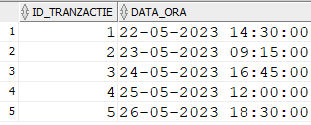
\includegraphics{images/inserare7.png}}
      \caption{ Inserare 7.}
    \end{figure}
    \vspace{0.5cm}

    \item \textbf{PRODUS}
    \vspace{0.2cm}
    \begin{lstlisting}
CREATE TABLE PRODUS (
 id_produs NUMBER(4) PRIMARY KEY,
 nume_produs VARCHAR2(50),
 pret NUMBER(4),
 id_stoc NUMBER(4),
 id_tranzactie NUMBER(4),
 FOREIGN KEY (id_stoc) REFERENCES STOC (id_stoc),
 FOREIGN KEY (id_tranzactie) REFERENCES TRANZACTIE (id_tranzactie)
);
INSERT INTO PRODUS VALUES (1, 'Chec Pufos', 20, 4, 1);
INSERT INTO PRODUS VALUES (2, 'Tricou', 200, 4, 2);
INSERT INTO PRODUS VALUES (3, 'Pantaloni', 300, 3, 2);
INSERT INTO PRODUS VALUES (4, 'Adidasi', 700, 4, 4);
 INSERT INTO PRODUS VALUES (5, 'Lapte', 5, 4, 1);
    \end{lstlisting}
    \vspace{0.2cm}
    \begin{figure}[h]
      \centerline{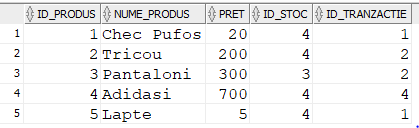
\includegraphics{images/inserare8.png}}
      \caption{ Inserare 8.}
    \end{figure}
    \vspace{0.5cm}

    \item \textbf{CLIENT}
    \vspace{0.2cm}
    \begin{lstlisting}
CREATE TABLE CLIENT (
 id_client NUMBER(4) PRIMARY KEY,
 nume_client VARCHAR2(40),
 email VARCHAR2(30) NOT NULL,
 telefon VARCHAR2(14)
);
INSERT INTO CLIENT VALUES (1, 'Ion Popescu', 'ion.popescu@example.com', '0721122334');
INSERT INTO CLIENT VALUES (2, 'Maria Ionescu', 'maria.ionescu@example.com', '0765432109');
INSERT INTO CLIENT VALUES (3, 'Ana Mihai', 'ana.mihai@example.com', '0755123456');
INSERT INTO CLIENT VALUES (4, 'Mihai Popa', 'mihai.popa@example.com', '0777555888');
INSERT INTO CLIENT VALUES (5, 'Elena Radu', 'elena.radu@example.com', '0744999222');
    \end{lstlisting}
    \vspace{0.2cm}
    \begin{figure}[h]
      \centerline{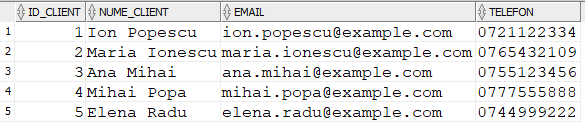
\includegraphics{images/inserare9.png}}
      \caption{ Inserare 9.}
    \end{figure}
    \vspace{0.5cm}

    \item \textbf{RECLAMATIE}
    \vspace{0.2cm}
    \begin{lstlisting}
CREATE TABLE RECLAMATIE (
 id_reclamatie NUMBER(4),
 data_ora TIMESTAMP,
 motiv VARCHAR2(1000),
 id_magazin NUMBER(4),
 id_client NUMBER(4),
 PRIMARY KEY (id_reclamatie, id_magazin, id_client),
 FOREIGN KEY (id_magazin) REFERENCES MAGAZIN (id_magazin),
 FOREIGN KEY (id_client) REFERENCES CLIENT (id_client)
);
INSERT INTO RECLAMATIE VALUES (1, TIMESTAMP '2023-05-22 10:30:00', 'Produs defect', 2, 3);
INSERT INTO RECLAMATIE VALUES (2, TIMESTAMP '2023-05-23 14:45:00', 'Serviciu neadecvat', 1,
4);
INSERT INTO RECLAMATIE VALUES (3, TIMESTAMP '2023-05-24 09:15:00', 'Reclamatie privind
preturile', 3, 2);
INSERT INTO RECLAMATIE VALUES (4, TIMESTAMP '2023-05-25 16:20:00', 'Produsului ii lipseste o
piesa', 1, 1);
INSERT INTO RECLAMATIE VALUES (5, TIMESTAMP '2023-05-26 11:10:00', 'Comportament angajat
neadecvat', 2, 5);
    \end{lstlisting}
    \vspace{0.2cm}
    \begin{figure}[h]
      \centerline{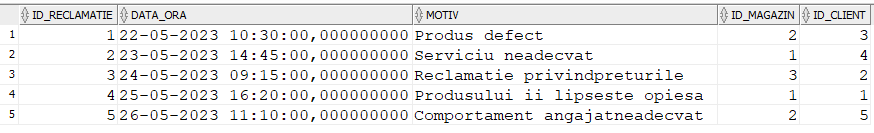
\includegraphics{images/inserare10.png}}
      \caption{ Inserare 10.}
    \end{figure}
    \vspace{0.5cm}

    \item \textbf{ACHIZITIE}
    \vspace{0.2cm}
    \begin{lstlisting}
CREATE TABLE ACHIZITIE (
 id_client NUMBER(4),
 id_magazin NUMBER(4),
 id_tranzactie NUMBER(4),
 PRIMARY KEY (id_client, id_magazin, id_tranzactie),
 FOREIGN KEY (id_magazin) REFERENCES MAGAZIN (id_magazin),
 FOREIGN KEY (id_tranzactie) REFERENCES TRANZACTIE (id_tranzactie),
 FOREIGN KEY (id_client) REFERENCES CLIENT (id_client)
);
INSERT INTO ACHIZITIE VALUES (1, 1, 1);
INSERT INTO ACHIZITIE VALUES (2, 2, 2);
INSERT INTO ACHIZITIE VALUES (3, 1, 3);
INSERT INTO ACHIZITIE VALUES (4, 3, 4);
INSERT INTO ACHIZITIE VALUES (5, 2, 5);
INSERT INTO ACHIZITIE VALUES (4, 1, 2);
INSERT INTO ACHIZITIE VALUES (2, 5, 3);
INSERT INTO ACHIZITIE VALUES (3, 4, 1);
INSERT INTO ACHIZITIE VALUES (5, 2, 4);
INSERT INTO ACHIZITIE VALUES (1, 3, 5);
    \end{lstlisting}
    \vspace{0.2cm}
    \begin{figure}[h]
      \centerline{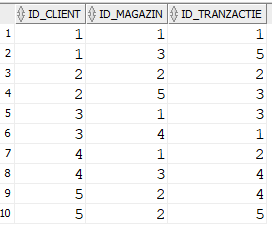
\includegraphics{images/inserare11.png}}
      \caption{ Inserare 11.}
    \end{figure}
    \vspace{0.5cm}

    \item \textbf{ANGAJAT}
    \vspace{0.2cm}
    \begin{lstlisting}
CREATE TABLE ANGAJAT (
 id_angajat NUMBER(4) PRIMARY KEY,
 nume_angajat VARCHAR2(30),
 salariu NUMBER(4),
 data_angajarii DATE
);
INSERT INTO ANGAJAT VALUES(1, 'Ion Popescu', 3000, TO_DATE('2022-01-15', 'YYYY-MM-DD'));
INSERT INTO ANGAJAT VALUES(2, 'Maria Ionescu', 2500, TO_DATE('2022-02-01', 'YYYY-MM-DD'));
INSERT INTO ANGAJAT VALUES(3, 'Alexandru Stanescu', 3500, TO_DATE('2022-03-10', 'YYYY-MMDD'));
INSERT INTO ANGAJAT VALUES(4, 'Elena Dumitrescu', 2800, TO_DATE('2022-04-05', 'YYYY-MM-DD'));
INSERT INTO ANGAJAT VALUES(5, 'Mihai Radu', 3200, TO_DATE('2022-05-20', 'YYYY-MM-DD'));
INSERT INTO ANGAJAT VALUES(6, 'Ana Vasilescu', 2700, TO_DATE('2022-06-11', 'YYYY-MM-DD'));
INSERT INTO ANGAJAT VALUES(7, 'Constantin Moldovan', 2900, TO_DATE('2022-07-02', 'YYYY-MMDD'));
INSERT INTO ANGAJAT VALUES(8, 'Andreea Nicolescu', 3100, TO_DATE('2022-08-18', 'YYYY-MM-DD'));
INSERT INTO ANGAJAT VALUES(9, 'George Marin', 2600, TO_DATE('2022-09-07', 'YYYY-MM-DD'));
INSERT INTO ANGAJAT VALUES(10, 'Simona Gheorghe', 3000, TO_DATE('2022-10-25', 'YYYY-MM-DD'));
INSERT INTO ANGAJAT VALUES(11,'Razvan Marian', 3500, TO_DATE('2018-05-29', 'YYYY-MM-DD'));
    \end{lstlisting}
    \vspace{0.2cm}
    \begin{figure}[h]
      \centerline{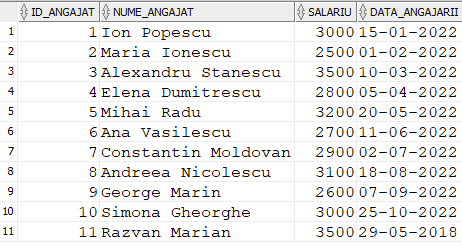
\includegraphics{images/inserare12.png}}
      \caption{ Inserare 12.}
    \end{figure}
    \vspace{0.5cm}

    \item \textbf{PAZNIC}
    \vspace{0.2cm}
    \begin{lstlisting}
CREATE TABLE PAZNIC (
 id_paznic NUMBER(4),
 norma VARCHAR2(20),
 id_angajat NUMBER(4) UNIQUE,
 id_firma NUMBER(4),
 PRIMARY KEY (id_angajat, id_paznic),
 FOREIGN KEY (id_angajat) REFERENCES ANGAJAT (id_angajat),
 FOREIGN KEY (id_firma) REFERENCES FIRMA (id_firma)
);
INSERT INTO PAZNIC VALUES(1, 'Norma intreaga', 1,1);
INSERT INTO PAZNIC VALUES(2, 'Norma intreaga', 3,2);
INSERT INTO PAZNIC VALUES(3, 'Part-time', 2,2);
INSERT INTO PAZNIC VALUES(4, 'Part-time', 5,3);
INSERT INTO PAZNIC VALUES(5, 'Norma intreaga', 4,5);
INSERT INTO PAZNIC VALUES(6,'Norma intreaga', 11, 3);
    \end{lstlisting}
    \vspace{0.2cm}
    \begin{figure}[h]
      \centerline{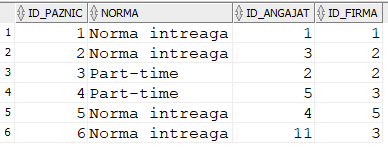
\includegraphics{images/inserare13.png}}
      \caption{ Inserare 13.}
    \end{figure}
    \vspace{0.5cm}

    \item \textbf{INTERN}
    \vspace{0.2cm}
    \begin{lstlisting}
CREATE TABLE INTERN (
 id_intern NUMBER(4),
 tura VARCHAR2(20),
 id_angajat NUMBER(4) UNIQUE,
 PRIMARY KEY (id_angajat, id_intern),
 id_magazin NUMBER(4),
 FOREIGN KEY (id_angajat) REFERENCES ANGAJAT (id_angajat),
 FOREIGN KEY (id_magazin) REFERENCES MAGAZIN (id_magazin)
);
INSERT INTO INTERN VALUES(1, 'Zi', 6,1);
INSERT INTO INTERN VALUES(2, 'Zi', 8,2);
INSERT INTO INTERN VALUES(3, 'Noapte', 7,3);
INSERT INTO INTERN VALUES(4, 'Noapte', 10,4);
INSERT INTO INTERN VALUES(5, 'Noapte', 9,5);
    \end{lstlisting}
    \vspace{0.2cm}
    \begin{figure}[h]
      \centerline{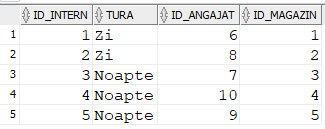
\includegraphics{images/inserare14.png}}
      \caption{ Inserare 14.}
    \end{figure}
    \vspace{0.5cm}
\end{itemize}


\addcontentsline{toc}{section}{Exercițiul 12}
\section*{12. Formulati in limbaj natural si implementati 5 cereri SQL complexe ce vor utiliza, in ansamblul lor, urmatoarele elemente:}

\vspace{0.5cm}
\begin{itemize}
    \item 
    \begin{lstlisting}
/*
 O cerere nesincronizata care afiseaza
toti chiriasii a caror magazine nu au nicio reclamatie.

-cerere sincronizata cu cel putin 3 tabele
-clauza WITH
*/

WITH Subcerere AS (
 SELECT m.id_chirias
 FROM MAGAZIN m
 LEFT JOIN RECLAMATIE r ON m.id_magazin = r.id_magazin
 WHERE r.id_magazin IS NULL
)
SELECT c.nume_chirias
FROM CHIRIAS c
WHERE c.id_chirias IN (
 SELECT id_chirias
 FROM Subcerere
);
    \end{lstlisting}
    \vspace{0.2cm}
    \begin{figure}[h]
      \centerline{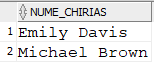
\includegraphics{images/interogare1.png}}
      \caption{ Interogare 1.}
    \end{figure}
    \vspace{0.5cm}

    \item 
    \begin{lstlisting}
/*
 Afisarea tuturor magazinelor a caror mall detine o promovare, selectand
astfel numele magazinului (cu majuscule), data cand incepe campania de promovare
(in format zi-luna-an), data cand se sfarseste campania (in format an-luna-zi), verificandu-se daca este un magazin profitabil (profitul>5000), si daca are un nume lung sau scurt(sa fie de maxim 9 caractere).

-functii cu siruri de caractere/data
-case
*/

SELECT
 UPPER(m.nume_magazin) AS nume_magazin,
 TO_CHAR(p.data_inceput, 'DD-MON-YYYY') AS data_inceput,
 TO_CHAR(p.data_sfarsit, 'YYYY-MM-DD') AS data_sfarsit,
 CASE
 WHEN m.profit_lunar > 5000 THEN 'Profitabil'
 ELSE 'Neprofitabil'
 END AS situatie_profit,
 CASE
 WHEN LENGTH(m.nume_magazin) > 9 THEN 'Nume Lung'
 ELSE 'Nume Scurt'
 END AS lungime_nume
FROM MAGAZIN m
JOIN MALL ma ON m.id_mall = ma.id_mall
JOIN PROMOVARE p ON ma.id_promovare = p.id_promovare
WHERE ma.id_promovare IS NOT NULL;
    \end{lstlisting}
    \vspace{3cm}
    \begin{figure}[h]
      \centerline{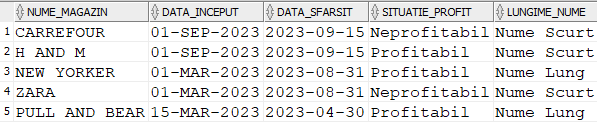
\includegraphics{images/interogare2.png}}
      \caption{ Interogare 2.}
    \end{figure}
    \vspace{0.5cm}

    \item 
    \begin{lstlisting}
/*
 Afisarea tuturor magazinelor care au profitul lunar mai mare de 5000.

 -Functii grup ( GROUP BY, HAVING)
*/
SELECT nume_magazin, SUM(profit_lunar) AS profit_total
FROM MAGAZIN
GROUP BY nume_magazin
HAVING SUM(profit_lunar) > 5000
    \end{lstlisting}
    \vspace{0.2cm}
    \begin{figure}[h]
      \centerline{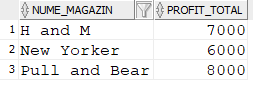
\includegraphics{images/interogare3.png}}
      \caption{ Interogare 3.}
    \end{figure}
    \vspace{0.5cm}


    \item 
    \begin{lstlisting}
/*
Sa se afiseze toti paznicii (id-ul, numele_angajatului) si firma la care lucreaza care au o norma intreaga.

-subcerere nesincronizata in FROM
*/

SELECT p.id_paznic, a.nume_angajat, f.nume_firma
FROM (SELECT * FROM PAZNIC WHERE norma = 'Norma intreaga') p, FIRMA f, ANGAJAT a
WHERE p.id_firma = f.id_firma
AND p.id_angajat = a.id_angajat
    \end{lstlisting}
    \vspace{0.2cm}
    \begin{figure}[h]
      \centerline{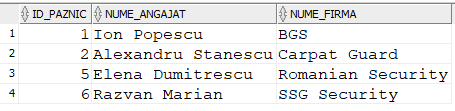
\includegraphics{images/interogare4.png}}
      \caption{ Interogare 4.}
    \end{figure}
    \vspace{0.5cm}

    \item 
    \begin{lstlisting}
/*
Sa se afiseze toate mall-urile, cu campaniile de promovare (numele mall-ului, numele campaniei, data de incepere, si data de sfarsit) In cazul in care mall-ul nu are campanie se va afisa "Fara campanie", iar la data de inceput si sfarsit "Informatie indisponibila"

-DECODE
*/
SELECT m.nume_mall, NVL(p.nume_campanie, 'Fara campanie') AS nume_campanie,
 DECODE(p.data_inceput, NULL, 'Informatie indisponibila', TO_CHAR(p.data_inceput, 'DDMM-YYYY')) AS data_inceput,
 DECODE(p.data_sfarsit, NULL, 'Informatie indisponibila', TO_CHAR(p.data_sfarsit, 'DDMM-YYYY')) AS data_sfarsit
FROM MALL m
LEFT JOIN PROMOVARE p ON m.id_promovare = p.id_promovare;
    \end{lstlisting}
    \vspace{0.2cm}
    \begin{figure}[h]
      \centerline{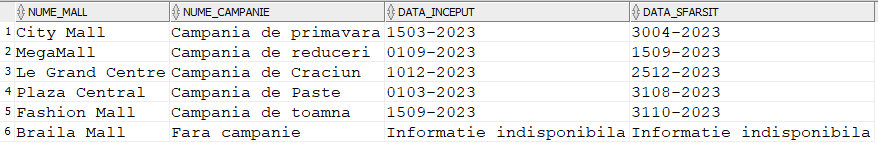
\includegraphics{images/interogare5.png}}
      \caption{ Interogare 5.}
    \end{figure}
    \vspace{0.5cm}
\end{itemize}


\addcontentsline{toc}{section}{Exercițiul 13}
\section*{13. Implementarea a 3 operatii de actualizare si de suprimare a datelor utilizand subcereri.}
\vspace{0.5cm}
\begin{itemize}
    \item 
    \begin{lstlisting}
UPDATE MALL
SET nume_mall = 'Roby Mall'
WHERE id_mall IN ( SELECT m.id_mall
 FROM MALL m
 JOIN PROMOVARE p ON m.id_promovare = p.id_promovare
 WHERE p.nume_campanie = 'Campania de primavara');
    \end{lstlisting}
    \vspace{0.5cm}
    \item 
    \begin{lstlisting}
UPDATE MALL
SET dimensiune = dimensiune + 100
WHERE id_mall IN ( SELECT id_mall
 FROM PROMOVARE
 WHERE data_sfarsit < TO_DATE('2023-09-01', 'YYYY-MM-DD'));
    \end{lstlisting}
    \vspace{0.5cm}
    \item 
    \begin{lstlisting}
DELETE FROM PRODUS
WHERE pret < (
 SELECT AVG(pret) FROM PRODUS
)-45;
    \end{lstlisting}
\end{itemize}


\addcontentsline{toc}{section}{Exercițiul 14}
\section*{14. Formulati in limbaj natural si implementati in SQL:}

\vspace{0.5cm}
\begin{enumerate}
    \item \textbf{O cerere ce utilizeaza operatia outerjoin pe minimum 4 tabele.}
    \begin{lstlisting}
/*
Afisati id-ul, numele si email-ul persoanelor care au facut o reclamatie (in primavara) in magazinele care au profitul lunar mai mare de 3000, si a caror chirias este "Jane Smith".

*/

SELECT c.id_client, c.nume_client, c.email
FROM CLIENT c
FULL OUTER JOIN RECLAMATIE r ON c.id_client = r.id_client
FULL OUTER JOIN MAGAZIN m ON r.id_magazin = m.id_magazin
FULL OUTER JOIN CHIRIAS ch ON m.id_chirias = ch.id_chirias
WHERE r.data_ora >= TO_DATE('2023-03-01', 'YYYY-MM-DD') AND r.data_ora < TO_DATE('2023-06-01',
'YYYY-MM-DD')
 AND m.profit_lunar > 3000
 AND ch.nume_chirias = 'Jane Smith';
    \end{lstlisting}
    \vspace{0.2cm}
    \begin{figure}[h]
      \centerline{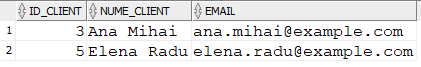
\includegraphics{images/interogare6.png}}
      \caption{ Interogare 6.}
    \end{figure}
    \vspace{0.5cm}

    \item \textbf{O cerere ce utilizează operatia division.}
    \begin{lstlisting}
/*
Afisati toate magazinele care vand doar pantaloni.

*/
SELECT m.nume_magazin
FROM MAGAZIN m
JOIN STOC s ON m.id_magazin = s.id_magazin
JOIN PRODUS p ON s.id_stoc = p.id_stoc
GROUP BY m.id_magazin, m.nume_magazin
HAVING COUNT(DISTINCT p.nume_produs) = 1
AND COUNT(DISTINCT CASE WHEN p.nume_produs = 'Pantaloni' THEN p.nume_produs END) = 1;
    \end{lstlisting}
    \vspace{0.2cm}
    \begin{figure}[h]
      \centerline{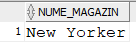
\includegraphics{images/interogare7.png}}
      \caption{ Interogare 7.}
    \end{figure}
    \vspace{0.5cm}

    \item \textbf{O cerere care implementează analiza top-n.}
    \begin{lstlisting}
/*
Top 3 magazine in functie de profit.

*/
SELECT *
FROM (
 SELECT m.id_magazin, m.nume_magazin, m.profit_lunar
 FROM MAGAZIN m
 ORDER BY m.profit_lunar DESC
)
WHERE ROWNUM <= 3;

    \end{lstlisting}
    \vspace{0.2cm}
    \begin{figure}[h]
      \centerline{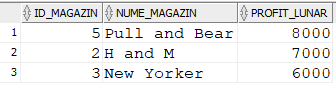
\includegraphics{images/interogare8.png}}
      \caption{ Interogare 8.}
    \end{figure}
\end{enumerate}


\end{document}
